\section{Question}

\textbf{Homologues} are two genes from a common ancestor DNA sequence which are related to each other. Furthermore, homologues can be classified as \textbf{Orthologues} or as \textbf{Paralogues}, whether they have been separated by the event of \textit{speciation} or by the event of \textit{genetic duplication}, respectively.

\subsection{Use a BLAST query to find orthologues of your gene. Describe what this query returned, and how you selected potential orthologues.}


I have run a Protein BLAST for the \href{https://www.ncbi.nlm.nih.gov/gene/3064}{\textit{huntingtin} [Homo sapiens]} protein (NCBI Reference Sequence: NP\_002102.4) - figure \ref{fig:htt-blastp-results} is a screenshot of some of the query results.

\begin{figure}[ht]
    \centering
    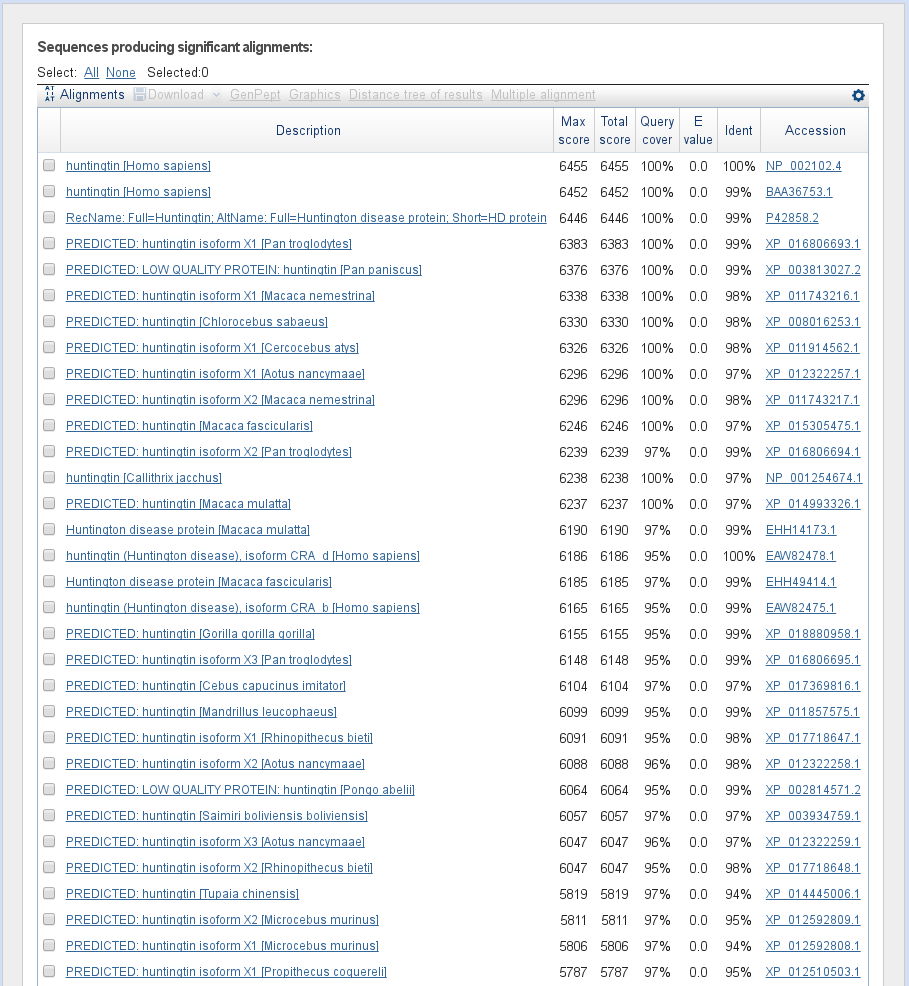
\includegraphics[width=\linewidth]{res/htt-blastp-results.png}
    \caption{Some of the \textit{htt} Protein BLAST results.}
    \label{fig:htt-blastp-results}
\end{figure}

The Protein BLAST query returned a list of sequences producing significant alignments, and a graphic summary with their alignment scores.

From this list we can select potential orthologues like: \textit{Pan troglodytes}, \textit{Macaca nemestrina}, \textit{Gorilla gorilla gorilla}, etc.

% - - - - - - - - - - - - - - - - - - - - - - - - - - -

\subsection{Compare your result with a query for homologues. To find these, select 'HomoloGene' in NCBI instead of 'Gene' as search option.}
\label{homologene-results}

HomoloGene \textit{huntingtin} query: \url{https://www.ncbi.nlm.nih.gov/homologene/1593}

The query linked above identifies the list below as being putative homologue genes:

\begin{multicols}{3}
    \begin{itemize}
        \item \textit{H. sapiens}
        \item \textit{P. troglodytes}
        \item \textit{C. lupus}
        \item \textit{B. taurus}
        \item \textit{M. musculus}
        \item \textit{R. norvegicus}
        \item \textit{G. gallus}
        \item \textit{X. tropicalis}
        \item \textit{D. rerio}
    \end{itemize}
\end{multicols}

% - - - - - - - - - - - - - - - - - - - - - - - - - - -

\subsection{How well do the results match when you consider e-value, percentage overlap, or score from your BLAST search?}

The following table contains the homologues returned by the HomoloGene query, and their respective \textit{E value}, \textit{query cover}, and \textit{score}, obtained by cross referencing their proteins \textit{accession} with the Protein BLAST results.

\begin{center}
	\begin{tabu} to \textwidth{ | X[c] | X[c] | X[c] | X[c] | }
		\hline
		Species & E value & Query cover & Score \\
		\hline
        \textit{H. sapiens}     & 0.0 & 100\% & 6455 \\
        \textit{P. troglodytes} & 0.0 & 100\% & 6383 \\
        \textit{C. lupus}       & 0.0 &  97\% & 5700 \\
        \textit{B. taurus}      & 0.0 &  97\% & 5579 \\
        \textit{M. musculus}    & 0.0 &  97\% & 5665 \\
        \textit{R. norvegicus}  & 0.0 &  97\% & 5671 \\
        \textit{G. gallus}      & 0.0 & 100\% & 5295 \\
        \textit{X. tropicalis}  & 0.0 &  99\% & 4949 \\
        \textit{D. rerio}       & 0.0 &  99\% & 4467 \\
		\hline
	\end{tabu}
\end{center}

\bigskip

\textbf{E value}

From the \href{https://blast.ncbi.nlm.nih.gov/blast/Blast.cgi?CMD=Web&PAGE_TYPE=BlastDocs&DOC_TYPE=FAQ#expect}{BLAST Frequently Asked questions}: \textit{The Expect value (E) is a parameter that describes the number of hits one can "expect" to see by chance when searching a database of a particular size. It decreases exponentially as the Score (S) of the match increases. Essentially, the E value describes the random background noise.}

Concerning our search results, all the results from the HomoloGene have a E value of 0.0, meaning they are all significant. Nonetheless, this indicator is no good for any comparison between the results.

\bigskip

\textbf{Percentage overlap}

By inspecting the table above, we can see that only three species - \textit{H. sapiens}, \textit{P. troglodytes}, and \textit{G. gallus} - have a total percentage overlap, i.e. query cover of 100\%.

\bigskip

\textbf{Score}

\textit{H. sapiens} is unsurprisingly the Species with the greatest score because we used it to run the HomoloGene query.

\textit{P. troglodytes} follows it, having a score of \textbf{6383}.

The species which has the next greatest score is \textit{R. norvegicus} - \textbf{5671}. Even though its query cover is only 97\%, its \textit{identity percentage} is greater than that of the other species of the table, which explains the higher score.

% - - - - - - - - - - - - - - - - - - - - - - - - - - -

\subsection{List those results from your initial query that you think are true orthologues, and explain why.}

\textbf{Note that NCBI BLAST has a useful view called 'Taxonomy Reports'. In addition to the NCBI service, you can also try the Ensembl database at \url{http://www.ensembl.org/Homo_sapiens/Tools/Blast?db=core.}}

Figure \ref{fig:blastp-taxonomy-view} shows the lineage tree obtained from the Protein BLAST search.

The following organisms are listed under \textit{Homininae}:

\begin{multicols}{2}
    \begin{itemize}
        \item \textit{Homo sapiens}
        \item \textit{Pan troglodytes}
        \item \textit{Pan paniscus}
        \item \textit{Gorilla gorilla gorilla}
    \end{itemize}
\end{multicols}

They constitute what I consider to be true orthologues for the \textit{huntingtin} gene.

\newpage

\begin{figure}[ht]
    \centering
    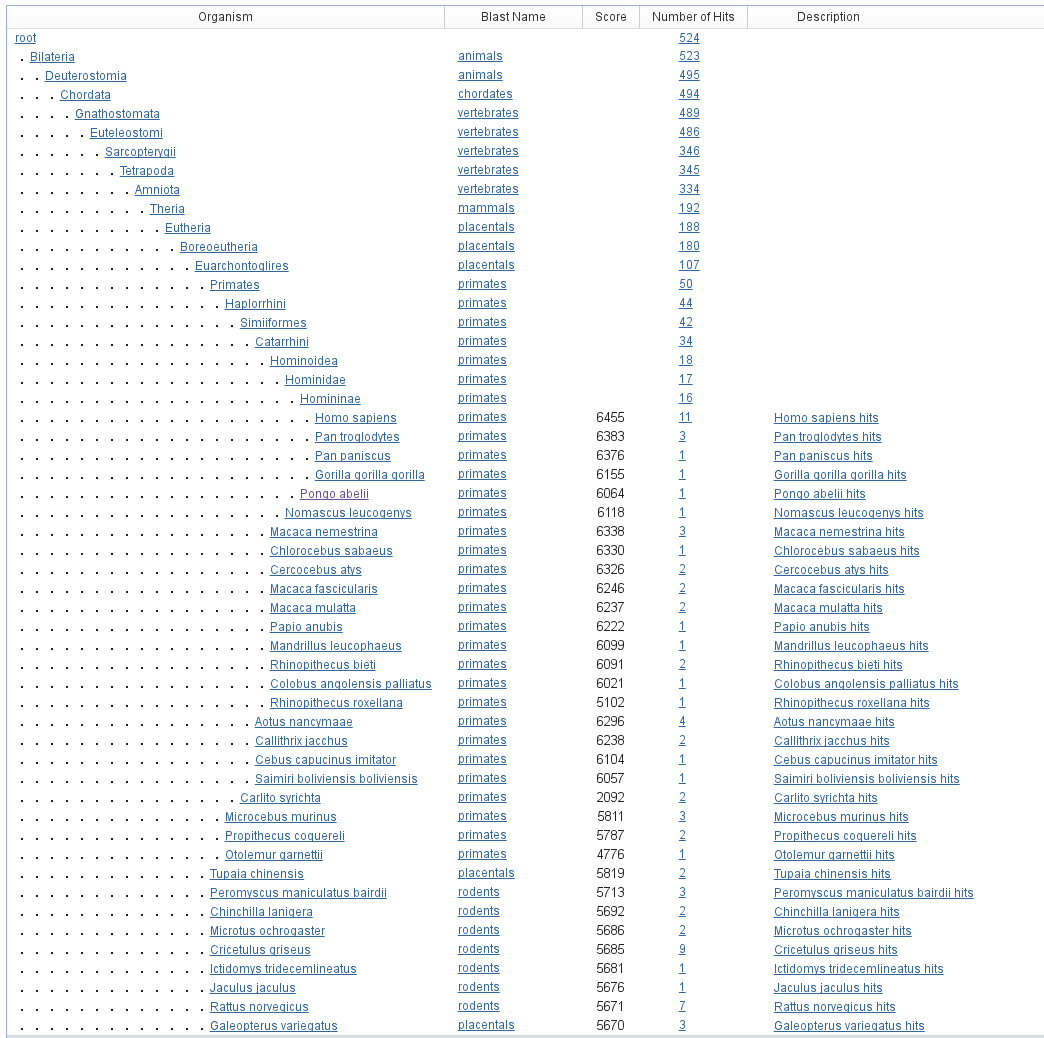
\includegraphics[width=\linewidth]{res/blastp-taxonomy-view.png}
    \caption{Screenshot of the taxonomy reports view from the \textit{htt} Protein BLAST results.}
    \label{fig:blastp-taxonomy-view}
\end{figure}

\newpage
